\chapter{द्रव्यमान स्पेक्ट्रममिति और परमाण्वीय स्पेक्ट्रमिकी}\label{ch:b2:mass-spec-atomic}

आतिशबाज़ी स्ट्रॉन्शियम लवणों से लाल, बेरियम लवणों से हरी, सोडियम से पीली होती है: ज्वाला
परमाणुओं को ऐसे रंगों के प्रकाश में बदल देती है जो उन्हें पहचानते हैं। द्रव्यमान स्पेक्ट्रममापी, दिखने में अधिक साधारण,
अकेले अणुओं को तौलता है, उन्हें उनके समस्थानिकों के अनुसार छाँटता है और उन्हें ऐसे टुकड़ों में तोड़ता है जिनके द्रव्यमान बताते हैं
कि वे कैसे बने थे। दोनों तकनीकें बहुत कम मात्राओं से प्रश्न ``इस नमूने में क्या है, और कितना?'' का उत्तर देती हैं,
पहली अणुओं के लिए, दूसरी तत्वों के लिए।

\begin{omfigure}

\includegraphics[width=0.58\linewidth]{images/book3/ai/b2-32-fireworks.jpg}

{\small नदी के ऊपर आतिशबाज़ी (चित्रण)। सोडियम का पीला रंग उसके परमाणुओं का प्रकाश है; गहरे
लाल और हरे रंग मुख्यतः ज्वाला में बने स्ट्रॉन्शियम और बेरियम के छोटे अणुओं से आते हैं।}
\end{omfigure}

\begin{recall}
विद्यालय का खंड: समस्थानिक और उनकी प्रचुरताएँ। प्रथम वर्ष का खंड: ऊर्जा स्तर और स्पेक्ट्रमी
रेखाएँ, अवशोषकता और बियर--लैम्बर्ट नियम, कार्बधनायन और मूलक, असंतृप्ति की मात्रा।
\Cref{ch:b2:chromatography}: \omterm{def:b2:chromatography:techniques}{गैस वर्णलेखन}, जो प्रायः किसी द्रव्यमान स्पेक्ट्रममापी को पोषित करता है।
\end{recall}

\section{द्रव्यमान स्पेक्ट्रममापी}

\begin{definition}[द्रव्यमान स्पेक्ट्रममिति]\label{def:b2:mass-spec-atomic:spectrum}
\emph{द्रव्यमान स्पेक्ट्रममिति}\index{द्रव्यमान स्पेक्ट्रममिति} किसी नमूने के अणुओं को गैसीय आयनों में बदलती है,
आयनों को उनके \emph{द्रव्यमान-आवेश अनुपात}\index{द्रव्यमान-आवेश अनुपात} $m/z$ के अनुसार पृथक करती है
(एकीकृत परमाणु द्रव्यमान इकाइयों में द्रव्यमान बटा आवेशों की संख्या) और उन्हें गिनती है।
\emph{द्रव्यमान स्पेक्ट्रम}\index{द्रव्यमान स्पेक्ट्रम} $m/z$ के विरुद्ध आयनों की प्रचुरता आलेखित करता है, प्रायः
आपेक्षिक तीव्रताओं के रूप में; उसका सबसे तीव्र शिखर, जिसे 100 माना जाता है, \emph{आधार शिखर}\index{आधार शिखर} है।
\end{definition}

स्पेक्ट्रममापी के तीन भाग होते हैं। स्रोत आयन बनाता है। इलेक्ट्रॉन आयनन (EI) में नमूने की वाष्प
\qty{70}{eV} के इलेक्ट्रॉनों की किरणपुंज को पार करती है, जो अणुओं से एक इलेक्ट्रॉन निकाल देते हैं और
उनमें अतिरिक्त ऊर्जा छोड़ देते हैं, जिससे अनेक अणु टूट जाते हैं। इलेक्ट्रोस्प्रे आयनन (ESI) में कोई विलयन
एक आवेशित सुई से फुहार के रूप में छोड़ा जाता है; बूँदों के वाष्पित होने पर अणु उन्हें एक अतिरिक्त प्रोटॉन
(या एक सोडियम आयन) के साथ, अक्षत, छोड़ देते हैं: बड़े, नाज़ुक अणुओं के लिए यही पसंदीदा विधि है। फिर विश्लेषक
आयनों को छाँटता है, और एक संसूचक उन्हें गिनता है।

\begin{omfigure}
\begin{tikzpicture}[x=1cm, y=1cm]
\draw[black!70, fill=omDef!10, rounded corners=2pt] (0,-0.6) rectangle (1.6,0.6);
\node[font=\small, align=center] at (0.8,0) {आयन\\स्रोत};
\draw[black!70] (2.0,-0.7) -- (2.0,0.7); \draw[black!70] (2.4,-0.7) -- (2.4,0.7);
\node[font=\footnotesize] at (2.2,1.0) {जालियाँ, $U$};
\draw[black!70] (2.6,-0.5) rectangle (8.4,0.5);
\node[font=\small] at (5.6,0.8) {क्षेत्र-मुक्त अपवाह नली, लंबाई $L$};
\draw[black!70, fill=black!15] (8.5,-0.6) rectangle (8.8,0.6);
\node[font=\small, align=center] at (9.6,0) {संसूचक};
\foreach \x/\c in {3.4/omThm, 4.6/omDef, 6.3/omMeth}{\fill[\c] (\x,0) circle (0.1);}
\draw[->, thick] (6.6,0) -- (7.4,0);
\node[font=\footnotesize, align=center] at (5.5,-0.85) {हल्के आयन आगे उड़ते हैं, भारी पीछे रहते हैं};
\end{tikzpicture}
\par\vspace{4pt}

{\small एक उड़ान-काल विश्लेषक (व्यवस्था-रूप)। समान विभवांतर
$U$ से त्वरित आयन समान गतिज ऊर्जा के साथ निकलते हैं; अपवाह नली में हल्के आयन तेज़ चलते हैं और पहले
संसूचक तक पहुँचते हैं।}
\end{omfigure}

\begin{proposition}[उड़ान काल]\label{prop:b2:mass-spec-atomic:time-of-flight}
द्रव्यमान $m$ और आवेश $ze$ का कोई आयन, विराम से विभवांतर $U$ द्वारा त्वरित होकर,
लंबाई $L$ की क्षेत्र-मुक्त नली को इतने समय में पार करता है:
\begin{equation*}
t = L\sqrt{\frac{m}{2zeU}}:
\end{equation*}
उड़ान काल $m/z$ के वर्गमूल के अनुसार बढ़ता है।
\end{proposition}

\begin{proof}
त्वरक क्षेत्र में ऊर्जा संरक्षण $\tfrac12mv^2 = zeU$ देता है, अतः $v = \sqrt{2zeU/m}$, और
नली नियत चाल से पार होती है: $t = L/v$।
\end{proof}

अन्य विश्लेषक आयनों को भिन्न ढंग से छाँटते हैं: चतुर्ध्रुव एक समय में केवल एक $m/z$ के आयनों को आगे जाने देता है,
जिन्हें चार छड़ों पर दोलायमान वोल्टताएँ चुनती हैं; चुंबकीय सेक्टर आयनों को ऐसे वृत्तों पर मोड़ता है जिनकी त्रिज्या
उनके संवेग पर निर्भर करती है। इन सभी में केवल $m/z$ मापा जाता है; EI द्वारा बने अधिकांश आयन एक
आवेश वहन करते हैं, अतः $m/z$ केवल उनका द्रव्यमान है।

\section{आण्विक आयन}

\begin{definition}[आण्विक और विखंड आयन]\label{def:b2:mass-spec-atomic:molecular-ion}
\emph{आण्विक आयन}\index{आण्विक आयन} $\mathrm M^{+\bullet}$ वह मूलक धनायन है जो तब बनता है जब कोई
अणु एक इलेक्ट्रॉन खोता है; उसका $m/z$ सबसे प्रचुर समस्थानिकों से बने अणु का
मोलर द्रव्यमान है। \emph{विखंड आयन}\index{विखंड आयन} आबंधों के टूटने से आण्विक आयन से
बनता है।
\end{definition}

\omterm{def:b2:mass-spec-atomic:molecular-ion}{आण्विक आयन} आण्विक द्रव्यमान देता है, जो किसी अज्ञात के बारे में पहला तथ्य है। EI में यह कभी-कभी दुर्बल या
अनुपस्थित होता है, जब \omterm{def:b2:mass-spec-atomic:molecular-ion}{आण्विक आयन} बहुत आसानी से टूट जाता है; तब इलेक्ट्रोस्प्रे, जो एक इकाई ऊपर $[\mathrm M +
\mathrm H]^+$ देता है, उसकी पुष्टि करता है।

\begin{definition}[नाइट्रोजन नियम]\label{def:b2:mass-spec-atomic:nitrogen-rule}
\emph{नाइट्रोजन नियम}\index{नाइट्रोजन नियम} कहता है कि किसी अणु का नाममात्र द्रव्यमान (उसके सबसे प्रचुर
समस्थानिकों की द्रव्यमान संख्याओं का योग) विषम होता है यदि और केवल यदि उसमें नाइट्रोजन परमाणुओं की
विषम संख्या हो।
\end{definition}

\begin{proposition}[नाइट्रोजन नियम की वैधता]\label{prop:b2:mass-spec-atomic:nitrogen-rule}
\omterm{def:b2:mass-spec-atomic:nitrogen-rule}{नाइट्रोजन नियम} C, H, N, O, S और हैलोजनों से बने ऐसे हर अणु के लिए सत्य है जिसमें कोई
अयुग्मित इलेक्ट्रॉन न हो।
\end{proposition}

\begin{proof}
नाममात्र द्रव्यमान C (12), N (14), O (16) और S (32) के लिए सम हैं, H (1) और हैलोजनों (19,
35, 79, 127) के लिए विषम। संयोजकताएँ C, O और S के लिए सम हैं, H, N और हैलोजनों के लिए विषम। अयुग्मित
इलेक्ट्रॉनों से रहित अणु में हर आबंध अपने दोनों परमाणुओं में से हर एक की एक संयोजकता प्रयुक्त करता है, अतः सभी
संयोजकताओं का योग सम है, और विषम संयोजकता वाले परमाणुओं की संख्या, $n_{\ce{H}} + n_{\ce{X}} + n_{\ce{N}}$,
सम है। नाममात्र द्रव्यमान की समता $n_{\ce{H}} + n_{\ce{X}}$ की समता है, जो इसलिए
$n_{\ce{N}}$ की समता है।
\end{proof}

\begin{definition}[समस्थानिक पैटर्न]\label{def:b2:mass-spec-atomic:isotope-pattern}
किसी आयन का \emph{समस्थानिक पैटर्न}\index{समस्थानिक पैटर्न} $M$, $M+1$,
$M+2$, \dots\ पर शिखरों का वह समूह है जो भारी समस्थानिकों वाले अणुओं से उत्पन्न होता है, और जिनकी तीव्रताएँ
उन समस्थानिक रूपों की प्रचुरताओं के अनुपात में होती हैं।
\end{definition}

\begin{proposition}[$M+1$ शिखर]\label{prop:b2:mass-spec-atomic:m-plus-one}
$n_C$ कार्बन परमाणुओं वाले और सार्थक $+1$ समस्थानिक वाले किसी अन्य तत्व से रहित आयन के लिए,
\begin{equation*}
\frac{I(M+1)}{I(M)} \approx n_C\,\frac{a_{13}}{a_{12}} \approx n_C \times 1.1~\%,
\end{equation*}
जहाँ $a_{12} = 0.989$ और $a_{13} = 0.011$ कार्बन के दोनों समस्थानिकों के मात्रा अंश हैं।
% ledger: iso:C12, iso:C13
\end{proposition}

\begin{proof}
सभी $n_C$ कार्बनों के \ce{^{12}C} होने की प्रायिकता $a_{12}^{n_C}$ है; ठीक एक के
\ce{^{13}C} होने की $n_C\,a_{13}a_{12}^{n_C - 1}$ (द्विपद नियम)। अनुपात $n_C\,a_{13}/a_{12}$ है, और
अन्य योगदान (दो \ce{^{13}C}, \ce{^2H}, \ce{^{15}N}) $a_{13}$ या उससे कम की कोटि के गुणक से
छोटे हैं।
\end{proof}

\begin{proposition}[क्लोरीन और ब्रोमीन]\label{prop:b2:mass-spec-atomic:halogen-patterns}
$p$ क्लोरीन और $q$ ब्रोमीन परमाणुओं वाले आयन के लिए $M$, $M+2$, $M+4$, \dots\ की तीव्रताएँ
$(a_{35} + a_{37}x)^p(a_{79} + a_{81}x)^q$ के, $x$ की घातों में, प्रसार के गुणांक हैं, जहाँ $x$ की हर
घात 2 द्रव्यमान इकाइयों को दर्शाती है। $a_{35} = 0.758$, $a_{37} = 0.242$, $a_{79} = 0.5069$ और
$a_{81} = 0.4931$ के साथ, एक क्लोरीन $M : M+2 \approx 3 : 1$ देता है और एक ब्रोमीन $\approx 1 : 1$।
% ledger: iso:Cl35, iso:Cl37, iso:Br79, iso:Br81
\end{proposition}

\begin{proof}
हर हैलोजन परमाणु स्वतंत्र रूप से हल्का समस्थानिक है या भारी, जो द्रव्यमान में 2 जोड़ता है। भारी परमाणुओं की
किसी दी गई संख्या $j$ की प्रायिकता प्रति परमाणु एक गुणक वाले गुणनफल में $x^j$ का गुणांक है,
जो बताया गया प्रसार है (प्रति तत्व द्विपद नियम)।
\end{proof}

\begin{omfigure}
\pgfplotsset{clu/.style={width=0.25\linewidth, height=3.3cm, ybar, bar width=5pt, ymin=0, ymax=118,
  xmin=-1.2, xmax=5.2, xtick={0,2,4}, xticklabels={$M$,$M\!+\!2$,$M\!+\!4$},
  tick label style={font=\tiny}, ytick=\empty, axis x line=bottom, axis y line=none,
  title style={font=\small, yshift=-4pt}, nodes near coords, nodes near coords style={font=\tiny},
  point meta=y, every node near coord/.append style={/pgf/number format/fixed, /pgf/number format/precision=0}}}
\begin{tikzpicture}
\begin{axis}[clu, title={Cl}]
\addplot[fill=omDef!55, draw=omDef, y filter/.expression={y==0 ? nan : y}] table[x=off, y=Cl] {figdata/out/bachelor-2-mass-spectra-a.dat};
\end{axis}
\end{tikzpicture}\hfill
\begin{tikzpicture}
\begin{axis}[clu, title={Cl$_2$}]
\addplot[fill=omDef!55, draw=omDef] table[x=off, y=Cl2] {figdata/out/bachelor-2-mass-spectra-a.dat};
\end{axis}
\end{tikzpicture}\hfill
\begin{tikzpicture}
\begin{axis}[clu, title={Br}]
\addplot[fill=omThm!45, draw=omThm, y filter/.expression={y==0 ? nan : y}] table[x=off, y=Br] {figdata/out/bachelor-2-mass-spectra-a.dat};
\end{axis}
\end{tikzpicture}\hfill
\begin{tikzpicture}
\begin{axis}[clu, title={Br$_2$}]
\addplot[fill=omThm!45, draw=omThm] table[x=off, y=Br2] {figdata/out/bachelor-2-mass-spectra-a.dat};
\end{axis}
\end{tikzpicture}\hfill
\begin{tikzpicture}
\begin{axis}[clu, title={ClBr}]
\addplot[fill=omMeth!45, draw=omMeth] table[x=off, y=ClBr] {figdata/out/bachelor-2-mass-spectra-a.dat};
\end{axis}
\end{tikzpicture}

{\small क्लोरीन और ब्रोमीन वाले आयनों के \omterm{def:b2:mass-spec-atomic:isotope-pattern}{समस्थानिक पैटर्न}, समस्थानिक
प्रचुरताओं से परिकलित (\cref{prop:b2:mass-spec-atomic:halogen-patterns}); हर समूह का सबसे तीव्र शिखर
100 माना गया है। ये पैटर्न अंगुलि-छाप हैं: एक क्लोरीन के लिए 3 : 1, एक ब्रोमीन के लिए 1 : 1, दो ब्रोमीन के लिए
1 : 2 : 1।}
% figdata: bachelor-2/mass-spectra.py part a
\end{omfigure}

\begin{definition}[यथातथ द्रव्यमान]\label{def:b2:mass-spec-atomic:exact-mass}
किसी आयन का \emph{एकसमस्थानिक द्रव्यमान}\index{एकसमस्थानिक द्रव्यमान} उसके सबसे प्रचुर
समस्थानिकों के यथातथ द्रव्यमानों का योग है (\ce{^{12}C} = ठीक 12, \ce{^1H} = 1.007825, \ce{^{16}O} = 15.994915,
\ce{^{14}N} = 14.003074 u)। \emph{उच्च-विभेदन द्रव्यमान स्पेक्ट्रममिति}\index{उच्च-विभेदन द्रव्यमान स्पेक्ट्रममिति}
$m/z$ को एक इकाई के कुछ हज़ारवें भाग या उससे बेहतर तक मापती है, जो समान
नाममात्र द्रव्यमान परंतु भिन्न सूत्रों वाले आयनों को अलग पहचानने के लिए पर्याप्त है।
% ledger: mass:C12, mass:H1, mass:O16, mass:N14
\end{definition}

\begin{proposition}[विभेदन क्षमता]\label{prop:b2:mass-spec-atomic:resolving}
द्रव्यमान $m$ और $m + \Delta m$ वाले दो आयन ऐसे विश्लेषक द्वारा पृथक होते हैं जिसकी विभेदन क्षमता कम-से-कम
$R = m/\Delta m$ हो। नाममात्र द्रव्यमान 28 पर \ce{CO+} (27.9949) को \ce{N2+} (28.0061) से पृथक करने के लिए $R
\approx 2.5 \times 10^3$ चाहिए; \ce{N2+} को \ce{C2H4+} (28.0313) से पृथक करने के लिए $R \approx 1.1 \times 10^3$।
\end{proposition}

\begin{proof}
विभेदन क्षमता $m/\Delta m$ के रूप में परिभाषित है, उस सबसे छोटे $\Delta m$ के लिए जिसे विश्लेषक पृथक करता है।
यथातथ द्रव्यमान समस्थानिक द्रव्यमानों से निकलते हैं: $12 + 15.994915$, $2 \times 14.003074$, $24 + 4 \times
1.007825$; फिर $28/(28.0061 - 27.9949) \approx 2.5 \times 10^3$ और $28/(28.0313 - 28.0061) \approx
1.1 \times 10^3$।
\end{proof}

\section{विखंडन}

EI द्वारा बना \omterm{def:b2:mass-spec-atomic:molecular-ion}{आण्विक आयन} किसी भी आबंध को तोड़ने के लिए आवश्यक ऊर्जा से कहीं अधिक ऊर्जा वहन करता है, और वह
उन पथों से टूटता है जो सबसे स्थायी उत्पाद देते हैं: स्थायीकृत धनायन, छोटे स्थायी उदासीन अणु या
मूलक। विखंडों को $M$ से हानियों के रूप में (\ce{CH3} के लिए 15, \ce{C2H5} या \ce{CHO} के लिए 29,
जल के लिए 18, CO या एथीन के लिए 28) और अभिलक्षणिक आयनों के रूप में पढ़ा जाता है।

\begin{definition}[दो विखंडन]\label{def:b2:mass-spec-atomic:fragmentation}
\emph{$\alpha$-विदलन}\index{अल्फ़ा-विदलन@$\alpha$-विदलन} में किसी विषमपरमाणु या किसी कार्बोनिल के बगल वाले कार्बन से
जुड़ा कोई आबंध टूटता है, जिससे विषमपरमाणु के एकाकी युग्म से स्थायीकृत एक धनायन बचता है (कीटोन के लिए
\omterm{def:b2:aromatic-substitution:friedel-crafts}{ऐसिलियम आयन} $\mathrm{R{-}C{\equiv}O^+}$, ऐमीन के लिए इमीनियम आयन)। किसी कार्बोनिल यौगिक का \emph{मैकलैफ़र्टी
पुनर्विन्यास}\index{मैकलैफ़र्टी पुनर्विन्यास} $\gamma$ कार्बन से एक हाइड्रोजन को कार्बोनिल ऑक्सीजन पर स्थानांतरित करता है
और $\alpha$--$\beta$ आबंध को तोड़ता है, जिससे एक ऐल्कीन और एक
\omterm{def:b2:enolates-aldol:tautomerism}{ईनॉल} मूलक धनायन मुक्त होते हैं।
\end{definition}

\begin{omfigure}
\begin{tikzpicture}
\begin{axis}[width=0.48\linewidth, height=4.6cm, xmin=10, xmax=80, ymin=0, ymax=118,
  xlabel={$m/z$}, ylabel={आपेक्षिक तीव्रता}, label style={font=\small}, tick label style={font=\scriptsize},
  title={\small ब्यूटेन-2-ओन}, ycomb, xtick={15,29,43,57,72}]
\addplot[omDef, thick] table[x=mz, y=I] {figdata/out/bachelor-2-mass-spectra-b.dat};
\node[font=\tiny, anchor=south] at (axis cs:43,100) {43};
\node[font=\tiny, anchor=south] at (axis cs:72,25) {72};
\node[font=\tiny, anchor=south] at (axis cs:57,8) {57};
\node[font=\tiny, anchor=south] at (axis cs:29,17) {29};
\end{axis}
\end{tikzpicture}\hfill
\begin{tikzpicture}
\begin{axis}[width=0.48\linewidth, height=4.6cm, xmin=10, xmax=140, ymin=0, ymax=118,
  xlabel={$m/z$}, ylabel={आपेक्षिक तीव्रता}, label style={font=\small}, tick label style={font=\scriptsize},
  title={\small 1-ब्रोमोप्रोपेन}, ycomb, xtick={27,43,79,107,122}]
\addplot[omThm, thick] table[x=mz, y=I] {figdata/out/bachelor-2-mass-spectra-c.dat};
\node[font=\tiny, anchor=south] at (axis cs:43,100) {43};
\node[font=\tiny, anchor=south] at (axis cs:123,9) {122, 124};
\node[font=\tiny, anchor=south] at (axis cs:27,26) {27};
\node[font=\tiny, anchor=south east] at (axis cs:40.5,31) {41};
\end{axis}
\end{tikzpicture}

{\small इलेक्ट्रॉन-आयनन स्पेक्ट्रम (NIST वेबबुक आँकड़े)। ब्यूटेन-2-ओन: \omterm{def:b2:mass-spec-atomic:molecular-ion}{आण्विक आयन} 72 पर;
$\alpha$-विदलन \omterm{def:b2:aromatic-substitution:friedel-crafts}{ऐसिलियम आयन} \ce{CH3CO+} (43, \omterm{def:b2:mass-spec-atomic:spectrum}{आधार शिखर}) और \ce{C2H5CO+} (57) देते हैं। 1-ब्रोमोप्रोपेन:
\omterm{def:b2:mass-spec-atomic:molecular-ion}{आण्विक आयन} 122 और 124 पर एक 1 : 1 युग्म है (\ce{^{79}Br}, \ce{^{81}Br}); ब्रोमीन परमाणु की हानि
43 पर \ce{C3H7+} छोड़ती है, जो \omterm{def:b2:mass-spec-atomic:spectrum}{आधार शिखर} है।}
% figdata: bachelor-2/mass-spectra.py parts b, c
% ledger: ms:butanone, ms:bromopropane
\end{omfigure}

\begin{omfigure}
\setchemfig{atom sep=1.8em}
\schemestart
\chemfig{[:-30]\chemabove{O}{\scriptstyle +\bullet}?[a]=[:-90]C(-[:-150]H_3C)-[:-30]CH_2-[:30]CH_2-[:90]CH_2-[:150]H?[a,1,{dash pattern=on 1pt off 1.5pt}]}
\arrow{->}[,1.0]
\chemfig{CH_2=C(-[2]OH)-CH_3}\,$^{+\bullet}$
\+
\chemfig{CH_2=CH_2}
\schemestop
\par\vspace{6pt}

{\small पेंटेन-2-ओन का \omterm{def:b2:mass-spec-atomic:fragmentation}{मैकलैफ़र्टी पुनर्विन्यास}, उसकी षट्सदस्यी चक्रीय
व्यवस्था से होकर खींचा गया: $\gamma$ कार्बन पर स्थित हाइड्रोजन ऑक्सीजन पर जाता है, $\alpha$--$\beta$ आबंध टूटता है,
एथीन निकलती है, और $m/z$ 58 पर प्रोपेनोन का \omterm{def:b2:enolates-aldol:tautomerism}{ईनॉल} मूलक धनायन बचता है।}
\end{omfigure}

\begin{proposition}[मैकलैफ़र्टी की आवश्यकता]\label{prop:b2:mass-spec-atomic:mclafferty}
\omterm{def:b2:mass-spec-atomic:fragmentation}{मैकलैफ़र्टी पुनर्विन्यास} के लिए $\gamma$ कार्बन पर एक हाइड्रोजन चाहिए। यह एक ऐल्कीन मुक्त करता है और
एक ऐसा मूलक धनायन छोड़ता है जिसके द्रव्यमान की समता आण्विक द्रव्यमान की समता जैसी होती है (नाइट्रोजन-रहित यौगिक के लिए
सम)।
\end{proposition}

\begin{proof}[तर्क]
हाइड्रोजन ऑक्सीजन, कार्बोनिल
कार्बन, $\alpha$, $\beta$ और $\gamma$ कार्बनों और स्वयं हाइड्रोजन की एक षट्सदस्यी चक्रीय व्यवस्था से होकर स्थानांतरित होता है: केवल $\gamma$ हाइड्रोजन
बिना तनाव के ऑक्सीजन तक पहुँचता है। बना आयन कार्बोनिल समूह, $\alpha$ कार्बन और
स्थानांतरित हाइड्रोजन को बनाए रखता है; जो निकलता है वह एक ऐल्कीन है, सम द्रव्यमान वाला उदासीन अणु, अतः आयन $M$ की
समता बनाए रखता है, जो उसे साधारण विदलनों से बने विषम-द्रव्यमान धनायनों से अलग करता है।
\end{proof}

\begin{method}[द्रव्यमान स्पेक्ट्रम पढ़ना]\label{met:b2:mass-spec-atomic:read-ms}
\begin{enumerate}
  \item \omterm{def:b2:mass-spec-atomic:molecular-ion}{आण्विक आयन} खोजिए (मुख्य समूह का उच्चतम $m/z$, जिसके नीचे तर्कसंगत हानियाँ हों)।
  \item उसका \omterm{def:b2:mass-spec-atomic:isotope-pattern}{समस्थानिक पैटर्न} पढ़िए: Cl, Br, S; $M+1$ शिखर कार्बनों की संख्या देता है।
  \item \omterm{def:b2:mass-spec-atomic:nitrogen-rule}{नाइट्रोजन नियम} लागू कीजिए; सूत्र और उनकी असंतृप्ति की मात्रा प्रस्तावित कीजिए।
  \item $M$ से हानियाँ और अभिलक्षणिक आयन पढ़िए (43 \ce{CH3CO+} या \ce{C3H7+}, 77
        \ce{C6H5+}, 91 \ce{C7H7+}, 105 \ce{C6H5CO+}); सम-द्रव्यमान मैकलैफ़र्टी आयन खोजिए।
  \item संरचनाएँ प्रस्तावित कीजिए; जाँचिए कि हर महत्त्वपूर्ण शिखर की व्याख्या हो।
\end{enumerate}
\end{method}

\section{परमाण्वीय स्पेक्ट्रमिकी}

परमाणुओं में कोई कंपन या घूर्णन नहीं होते; उनके स्पेक्ट्रम तीक्ष्ण रेखाएँ हैं, इलेक्ट्रॉनिक स्तरों के बीच
हर संक्रमण के लिए एक, तत्व की अभिलक्षणिक तरंगदैर्ध्यों पर। सोडियम ज्वाला का पीला रंग
\qty{589.0}{nm} और \qty{589.6}{nm} पर रेखाओं का युग्म है; लिथियम का किरमिजी रंग, \qty{670.8}{nm} पर एक रेखा;
स्ट्रॉन्शियम परमाणुओं की सबसे प्रबल रेखा \qty{460.7}{nm} पर है और बेरियम आयनों की
\qty{455.4}{nm} पर, नीले में: आतिशबाज़ी के लाल और हरे रंग मुख्यतः इन
धातुओं के अणुओं से आते हैं, उनके परमाणुओं से नहीं।
% ledger: asd:NaD2, asd:NaD1, asd:Li671, asd:Sr461, asd:Ba455

\begin{definition}[परमाण्वीय स्पेक्ट्रममितियाँ]\label{def:b2:mass-spec-atomic:atomic}
\emph{परमाण्वीय उत्सर्जन स्पेक्ट्रममिति}\index{परमाण्वीय उत्सर्जन स्पेक्ट्रममिति} में नमूने को किसी ज्वाला या प्लाज़्मा में
परमाणुकृत और उत्तेजित किया जाता है, और तत्व की किसी उत्सर्जन रेखा की तीव्रता मापी जाती है।
\emph{परमाण्वीय अवशोषण स्पेक्ट्रममिति}\index{परमाण्वीय अवशोषण स्पेक्ट्रममिति} (AAS) में नमूने को
किसी ज्वाला या ग्रेफ़ाइट भट्टी में परमाणुकृत किया जाता है और किसी अनुनाद रेखा पर परमाणुओं की अवशोषकता मापी जाती है,
जो एक \emph{खोखला-कैथोड लैंप}\index{खोखला-कैथोड लैंप} उत्सर्जित करता है जिसका कैथोड
स्वयं उसी तत्व का बना होता है। \emph{प्रेरणिक युग्मित प्लाज़्मा}\index{प्रेरणिक युग्मित प्लाज़्मा} (ICP) में
रेडियो-आवृत्ति क्षेत्र द्वारा कई हज़ार केल्विन तक गर्म किया गया आर्गन नमूने को परमाणुकृत और आयनित करता है;
प्लाज़्मा किसी उत्सर्जन स्पेक्ट्रममापी (ICP-OES) या द्रव्यमान स्पेक्ट्रममापी (ICP-MS) को पोषित करता है।
\end{definition}

\begin{omfigure}
\begin{tikzpicture}[x=1cm, y=1cm, box/.style={draw=black!70, rounded corners=2pt, fill=white,
  font=\small, align=center, minimum height=0.8cm, inner sep=3pt}]
\node[box] (lamp) at (0,0) {खोखला-कैथोड\\लैंप (Cu)};
\shade[top color=omThm!60, bottom color=omThm!10] (2.6,-0.25) -- (3.3,-0.25) -- (3.15,0.75) -- (2.75,0.75) -- cycle;
\draw[black!70, fill=black!15] (2.4,-0.45) rectangle (3.5,-0.25);
\node[font=\footnotesize] at (2.95,-0.75) {ज्वाला (परमाणु)};
\node[box] (mono) at (6.1,0) {एकवर्णित्र};
\node[box] (det) at (8.5,0) {संसूचक};
\node[box] (data) at (10.8,0) {अवशोषकता};
\draw[->, thick, omDef] (lamp.east) -- (mono.west);
\draw[->, thick] (mono) -- (det); \draw[->, thick] (det) -- (data);
\node[font=\footnotesize, omDef] at (4.4,0.3) {$I_0 \to I$};
\end{tikzpicture}
\par\vspace{4pt}

{\small एक परमाण्वीय अवशोषण स्पेक्ट्रममापी (व्यवस्था-रूप)। लैंप स्वयं कॉपर की रेखाएँ उत्सर्जित करता है, जिनमें
\qty{324.75}{nm} पर अनुनाद रेखा भी है; ज्वाला में कॉपर परमाणु उसे अवशोषित करते हैं, और
एकवर्णित्र संसूचक के लिए उस रेखा को पृथक करता है।}
% ledger: asd:Cu325
\end{omfigure}

\begin{proposition}[परमाण्वीय अवशोषण मात्रात्मक है]\label{prop:b2:mass-spec-atomic:aas}
सांद्रताओं के एक परास में, किसी अनुनाद रेखा पर मापी गई अवशोषकता ज्वाला में फुहारे गए विलयन में तत्व की
सांद्रता के समानुपाती होती है।
\end{proposition}

\admitted

यह मुक्त परमाणुओं पर लागू प्रथम वर्ष के खंड का बियर--लैम्बर्ट नियम है: ज्वाला विलयन के एक नियत
अंश को परमाणुओं में बदलती है, और लैंप रेखा, जो अवशोषण रेखा से संकरी है,
एकवर्णी प्रकाश की तरह व्यवहार करती है। उच्च सांद्रता पर रेखा संतृप्त हो जाती है और अंशांकन वक्र मुड़ जाता है, इसीलिए
कार्य-परास की जाँच की जाती है।

\begin{method}[परमाण्वीय अवशोषण मापन का अंशांकन]\label{met:b2:mass-spec-atomic:aas-calibration}
\begin{enumerate}
  \item अपेक्षित परास को ढकने वाले एक रिक्त और चार या पाँच मानक बनाइए, नमूनों जैसे ही अम्ल
        आधात्री में।
  \item चुनी गई रेखा पर उनकी अवशोषकताएँ मापिए; $A = a\,c$ (या $A = a\,c + b$) समंजित कीजिए;
        रैखिकता जाँचिए।
  \item नमूनों को मापिए, आवश्यक हो तो परास के भीतर लाने के लिए तनु करके; $c = (A - b)/a$ परिकलित कीजिए।
  \item अपवाह जाँचने के लिए अंत में एक मानक फिर मापिए; हर तनुकरण के लिए संशोधन कीजिए।
\end{enumerate}
\end{method}

ICP-MS सबसे निम्न सांद्रताओं तक पहुँचता है, परंतु उसके आयन द्रव्यमान में समान
नाममात्र द्रव्यमान वाले अन्य आयनों से टकरा सकते हैं: प्लाज़्मा गैस से बना \ce{^{40}Ar^{16}O+} \ce{^{56}Fe+} पर पड़ता है, और \ce{^{40}Ar+}
\ce{^{40}Ca+} पर। उच्च-विभेदन विश्लेषक, संघट्ट सेल या विश्लेष्य का कोई अन्य समस्थानिक
व्यतिकरण को हटा देता है। संसूचन सीमाएँ, और उन्हें कैसे मापा जाए, \cref{ch:b2:measurement-statistics}
का विषय हैं।

\begin{history}[परमाणुओं को तौलना, तत्वों को देखना]
\begin{minipage}[t]{0.17\linewidth}
\vspace{0pt}
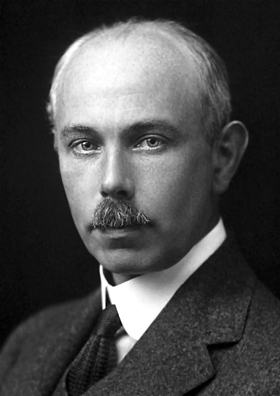
\includegraphics[width=\linewidth]{images/book3/aston.jpg}
\end{minipage}\hspace{0.02\linewidth}%
\begin{minipage}[t]{0.24\linewidth}
\vspace{0pt}
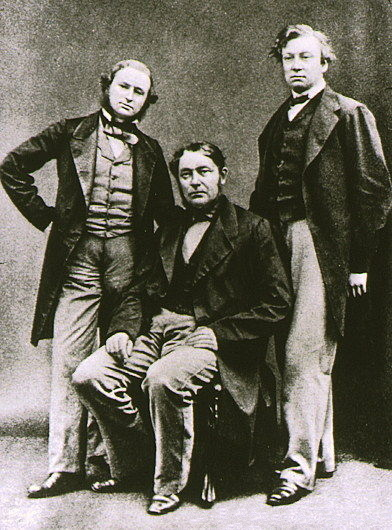
\includegraphics[width=\linewidth]{images/book3/kirchhoff-bunsen.jpg}
\end{minipage}\hfill
\begin{minipage}[t]{0.54\linewidth}
\vspace{0pt}
गुस्ताफ़ किरखॉफ़ और रॉबर्ट बुन्सन ने 1860 के आसपास दिखाया कि हर तत्व ज्वाला में अपनी रेखाएँ देता है,
और अपनी अज्ञात रेखाओं से सीज़ियम और रुबिडियम की खोज की। 1919 से फ़्रांसिस ऐस्टन के द्रव्यमान स्पेक्ट्रमलेखी ने
दिखाया कि अधिकांश तत्व समस्थानिकों के मिश्रण हैं; उन्हें 1922 का रसायन का नोबेल पुरस्कार मिला।
(छायाचित्र: ऐस्टन, अज्ञात लेखक, सार्वजनिक अधिकार-क्षेत्र; 1862 में किरखॉफ़, बुन्सन और हेनरी रॉस्को,
रॉस्को के संग्रह से, सार्वजनिक अधिकार-क्षेत्र; विकिमीडिया कॉमन्स।)
\end{minipage}
\end{history}

\section{अभ्यास}

\begin{exercise}[$\star$]\label{exo:b2:mass-spec-atomic:1}
इनका $m/z$ दीजिए: बेन्ज़ीन \ce{C6H6} का \omterm{def:b2:mass-spec-atomic:molecular-ion}{आण्विक आयन}; दो आवेश वहन करने वाला \qty{400}{u} द्रव्यमान का
एक आयन; इलेक्ट्रोस्प्रे द्वारा बना कैफ़ीन (\ce{C8H10N4O2}, नाममात्र द्रव्यमान 194) का प्रोटॉनित अणु।
\end{exercise}

\begin{exercise}[$\star$]\label{exo:b2:mass-spec-atomic:2}
C, H, N और O से बने किसी यौगिक का \omterm{def:b2:mass-spec-atomic:molecular-ion}{आण्विक आयन} $m/z$ 73 पर है। इसके नाइट्रोजन परमाणुओं के बारे में क्या कहा जा सकता है?
एक सूत्र प्रस्तावित कीजिए।
\end{exercise}

\begin{exercise}[$\star$]\label{exo:b2:mass-spec-atomic:3}
एक आण्विक-आयन समूह दो इकाई की दूरी पर लगभग समान ऊँचाई के दो शिखर दिखाता है। दूसरा दो इकाई की दूरी पर
3 : 1 अनुपात में दो शिखर दिखाता है। कौन-से हैलोजन?
\end{exercise}

\begin{exercise}[$\star$]\label{exo:b2:mass-spec-atomic:4}
एक लवण ज्वाला को पीला रंग देता है; दूसरा किरमिजी। तत्वों को पहचानिए और उनकी रेखाओं की तरंगदैर्ध्य
दीजिए।
\end{exercise}

\begin{exercise}[$\star\star$]\label{exo:b2:mass-spec-atomic:5}
किसी हाइड्रोकार्बन का $M$ 100 \% पर और $M+1$ 6.7 \% पर है। इसमें कितने कार्बन परमाणु हैं?
\end{exercise}

\begin{exercise}[$\star\star$]\label{exo:b2:mass-spec-atomic:6}
\ce{CO}, \ce{N2} और \ce{C2H4} के यथातथ द्रव्यमान परिकलित कीजिए और हर युग्म को पृथक करने के लिए आवश्यक
विभेदन क्षमता भी।
\end{exercise}

\begin{exercise}[$\star\star$]\label{exo:b2:mass-spec-atomic:7}
पेंटेन-3-ओन का EI स्पेक्ट्रम 86, 57 (\omterm{def:b2:mass-spec-atomic:spectrum}{आधार शिखर}) और 29 पर शिखर दिखाता है। उन्हें निर्दिष्ट कीजिए।
\end{exercise}

\begin{exercise}[$\star\star$]\label{exo:b2:mass-spec-atomic:8}
पेंटेन-2-ओन का स्पेक्ट्रम 86, 71, 58 और 43 (\omterm{def:b2:mass-spec-atomic:spectrum}{आधार शिखर}) पर शिखर दिखाता है। उन्हें निर्दिष्ट कीजिए, और समझाइए
कि पेंटेन-3-ओन 58 पर केवल एक छोटा शिखर क्यों दिखाता है।
\end{exercise}

\begin{exercise}[$\star\star$]\label{exo:b2:mass-spec-atomic:9}
1.0, 2.0, 3.0 और \qty{4.0}{mg/L} पर कॉपर मानक अवशोषकताएँ 0.052, 0.104, 0.155 और 0.207 देते हैं;
एक नमूना 0.128 देता है (अभ्यास के आँकड़े)। इसकी कॉपर सांद्रता परिकलित कीजिए।
\end{exercise}

\begin{exercise}[$\star\star\star$]\label{exo:b2:mass-spec-atomic:10}
किसी उड़ान-काल विश्लेषक में $L = \qty{1.00}{m}$ और $U = \qty{20.0}{kV}$ है। \qty{1000}{u} द्रव्यमान वाले
एकल-आवेशित आयन का उड़ान काल परिकलित कीजिए, और \qty{1001}{u} वाले आयन से उसे अलग करने वाला समय भी।
\end{exercise}

\begin{exercise}[$\star\star\star$]\label{exo:b2:mass-spec-atomic:11}
डाइक्लोरोमेथेन, \ce{CH2Cl2}, का आण्विक-आयन समूह परिकलित कीजिए: $m/z$ मान और आपेक्षिक
तीव्रताएँ।
\end{exercise}

\begin{exercise}[$\star\star\star$]\label{exo:b2:mass-spec-atomic:12}
ICP-MS में \ce{^{40}Ar^{16}O+} \ce{^{56}Fe+} के साथ व्यतिकरण करता है। उन्हें पृथक करने के लिए आवश्यक विभेदन क्षमता परिकलित कीजिए,
और कोई अन्य उपाय प्रस्तावित कीजिए।
\end{exercise}

\section{समस्या: एक अज्ञात हैलाइड}

\begin{problem}[{सप्ताहांत समस्या --- क्लोरीन और ब्रोमीन वाला एक आण्विक-आयन समूह,
कार्बनों की संख्या, विखंड, और हर शिखर के विरुद्ध जाँची गई एक संरचना}]
\label{pb:b2:mass-spec-atomic:1}
एक रंगहीन द्रव, जो \omterm{def:b2:chromatography:techniques}{गैस वर्णलेखन} द्वारा एक ही शिखर के रूप में उत्क्षालित होता है, नीचे दिया गया EI \omterm{def:b2:mass-spec-atomic:spectrum}{द्रव्यमान स्पेक्ट्रम} देता है (NIST
वेबबुक आँकड़े)। मुख्य शिखर ($m/z$: आपेक्षिक तीव्रता): 156: 14.5; 157: 0.5; 158: 18.6; 159: 0.6; 160:
4.4; 107: 6.7; 109: 6.3; 93: 3.3; 95: 2.9; 77: 59; 79: 18.7; 76: 39.5; 49: 12.9; 51: 4.3; 41: 100; 39:
26.2; 27: 24.6। समस्थानिक प्रचुरताएँ: \ce{^{35}Cl} 0.758, \ce{^{37}Cl} 0.242, \ce{^{79}Br} 0.5069,
\ce{^{81}Br} 0.4931, \ce{^{12}C} 0.989, \ce{^{13}C} 0.011।
% ledger: ms:bromochloropropane, iso:Cl35, iso:Cl37, iso:Br79, iso:Br81, iso:C12, iso:C13, mass:C12, mass:H1, mass:Br79, mass:Cl35

\begin{center}
\begin{tikzpicture}
\begin{axis}[width=0.8\linewidth, height=4.6cm, xmin=20, xmax=170, ymin=0, ymax=112,
  xlabel={$m/z$}, ylabel={आपेक्षिक तीव्रता}, label style={font=\small},
  tick label style={font=\scriptsize}, ycomb, xtick={27,41,49,77,93,107,122,156}]
\addplot[omDef, thick] table[x=mz, y=I] {figdata/out/bachelor-2-mass-spectra-d.dat};
\end{axis}
\end{tikzpicture}
\end{center}
% figdata: bachelor-2/mass-spectra.py part d

\medskip
\noindent\textbf{भाग I --- \omterm{def:b2:mass-spec-atomic:molecular-ion}{आण्विक आयन}।}
\begin{enumerate}
  \item कौन-से शिखर आण्विक-आयन समूह बनाते हैं? यह एक अकेला शिखर क्यों नहीं है?
  \item 2 के अंतराल वाले तीन शिखरों का समूह किन हैलोजनों की ओर संकेत करता है?
  \item सबसे हल्के समस्थानिक रूप का नाममात्र द्रव्यमान क्या है?
  \item \omterm{def:b2:mass-spec-atomic:nitrogen-rule}{नाइट्रोजन नियम} क्या कहता है?
  \item एक \ce{^{79}Br} और एक \ce{^{35}Cl} घटाइए: क्या बचता है, और किस हाइड्रोकार्बन खंड का
        वह द्रव्यमान है?
  \item एक आण्विक सूत्र प्रस्तावित कीजिए और उसकी असंतृप्ति की मात्रा दीजिए।
\end{enumerate}

\medskip
\noindent\textbf{भाग II --- कार्बन और यथातथ द्रव्यमान।}
\begin{enumerate}[resume]
  \item 157/156 अनुपात से कार्बनों की संख्या का अनुमान लगाइए।
  \item यहाँ वह अनुमान मोटा क्यों है?
  \item 158 पर शिखर में कौन-से समस्थानिक रूप योगदान देते हैं?
  \item \omterm{def:b2:mass-spec-atomic:molecular-ion}{आण्विक आयन} का \omterm{def:b2:mass-spec-atomic:exact-mass}{एकसमस्थानिक द्रव्यमान} परिकलित कीजिए।
  \item \ce{C10H20O} का नाममात्र द्रव्यमान भी 156 है (यथातथ 156.151)। कौन-सी विभेदन क्षमता
        दोनों को पृथक करती है?
  \item क्या C=C आबंध और उन्हीं हैलोजनों वाले किसी यौगिक के \omterm{def:b2:mass-spec-atomic:molecular-ion}{आण्विक आयन} का नाममात्र द्रव्यमान
        भिन्न होगा?
\end{enumerate}

\medskip
\noindent\textbf{भाग III --- विखंड।}
\begin{enumerate}[resume]
  \item युग्म 77/79 3 : 1 के अनुपात में है। कौन-सा परमाणु खोया गया है, और आयन क्या है?
  \item 76 पर शिखर की व्याख्या कीजिए।
  \item 41 पर \omterm{def:b2:mass-spec-atomic:spectrum}{आधार शिखर} निर्दिष्ट कीजिए।
  \item युग्म 49/51 निर्दिष्ट कीजिए।
  \item युग्म 93/95 और 107/109 निर्दिष्ट कीजिए।
  \item ब्रोमीन परमाणु क्लोरीन परमाणु की तुलना में अधिक आसानी से क्यों खोया जाता है?
  \item 1-ब्रोमो-1-क्लोरोप्रोपेन 127, 129 और 131 पर \ce{CHBrCl+} देता। क्या स्पेक्ट्रम इसका
        समर्थन करता है?
\end{enumerate}

\medskip
\noindent\textbf{भाग IV --- संरचना।}
\begin{enumerate}[resume]
  \item संरचना प्रस्तावित कीजिए।
  \item जाँचिए कि यह सूचीबद्ध हर शिखर की व्याख्या करती है।
  \item क्या \omterm{def:b2:mass-spec-atomic:fragmentation}{मैकलैफ़र्टी पुनर्विन्यास} हो सकता है? क्यों?
  \item वह समावयवी खींचिए जो $m/z$ 63/65 पर प्रबल शिखर देता और 49/51 पर कोई नहीं।
  \item कौन-से समस्थानिक रूप 160 पर शिखर बनाते हैं?
  \item समस्थानिक प्रचुरताओं से एक क्लोरीन और एक ब्रोमीन के लिए $M$, $M+2$ और $M+4$ शिखरों का अनुपात
        परिकलित कीजिए, और स्पेक्ट्रम से उसकी तुलना कीजिए।
\end{enumerate}
\end{problem}
